% ============================================================
% Chapter 1: Introduction to Photovoltaic Systems and Fault Detection and Diagnosis Techniques
% ============================================================
\chapter{Background on Photovoltaic Systems}
\label{ch:pv-systems-fdd}

\section{Introduction}
\label{sec:pv-introduction}

This chapter presents the generalities of photovoltaic systems, including their operating principles and main components, followed by a description of the different faults that can occur in such installations. The final part introduces fault detection and diagnosis strategies that rely on electrical and meteorological sensor data to identify abnormal operating conditions and classify fault types in photovoltaic systems.

\section{Fundamentals of Photovoltaic Systems}
\label{sec:pv-fundamentals}

A photovoltaic (PV) system directly converts solar radiation into electricity via the photovoltaic effect. It primarily comprises PV modules to capture sunlight, inverters to convert direct current to alternating current, and protection devices for safe operation. Ranging from residential rooftops to utility-scale farms, a PV system's performance is driven by solar irradiance, ambient temperature, load characteristics, and cell technology \citep{alezz2022photovoltaic}.

\begin{figure}[H]
    \centering
    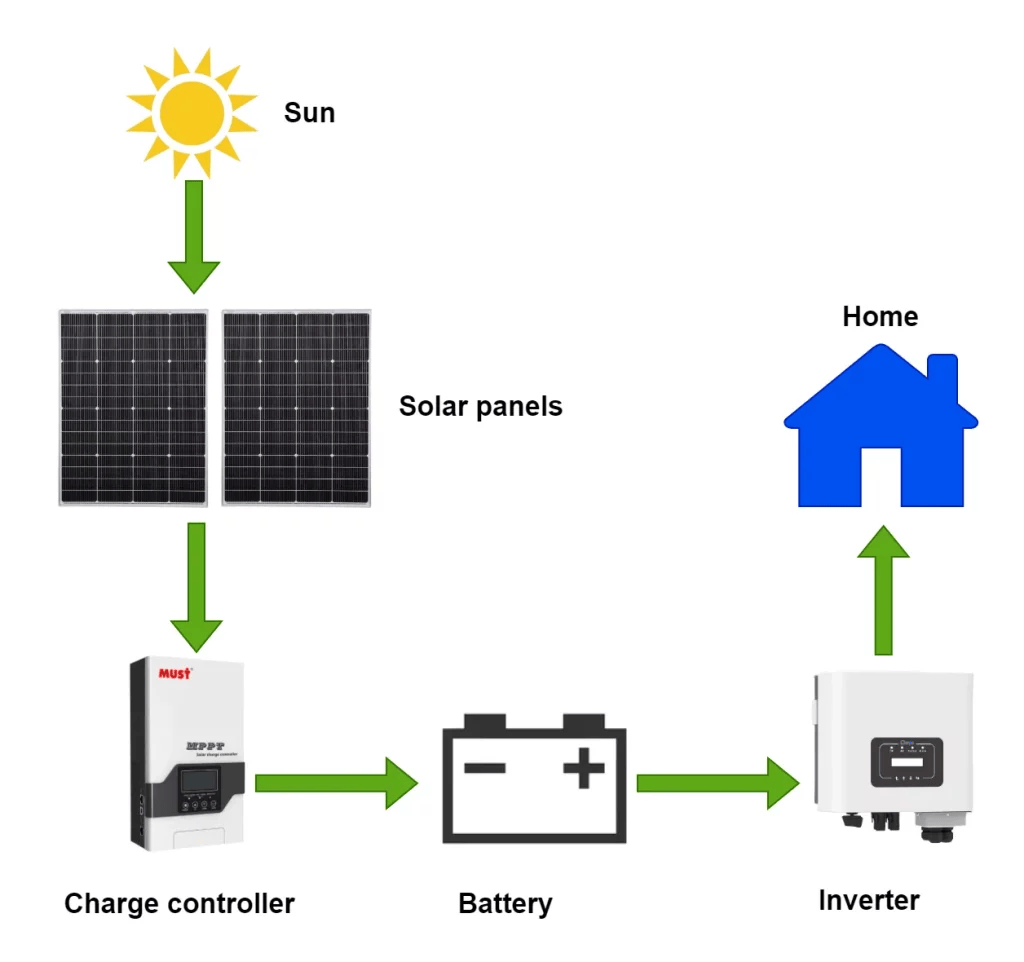
\includegraphics[width=0.4\textwidth]{figures/chap1/solar-system.png}
    \caption{Schematic of a Photovoltaic System}
    \label{fig:pv-system}
\end{figure}

\subsection{The Photovoltaic Effect}
\label{sec:pv-effect}

The photovoltaic effect, first observed by Edmond Becquerel in 1839, occurs when absorbed photons generate electron--hole pairs in a semiconductor p--n junction \citep{wurfel2016physics}. In silicon solar cells, this junction is formed by joining n-type and p-type regions, creating an internal electric field that separates photogenerated carriers and produces an external current under illumination \citep{marques2022photovoltaic}. Figure~\ref{fig:pv-effect} illustrates this principle \citep{energyeducation_pveffect}. The illuminated cell can be modeled by:
\begin{equation}
I = I_{\text{L}} - I_{0} \left[ \exp\left( \frac{q(V + I R_{\text{s}})}{n k_{\text{B}} T} \right) - 1 \right] - \frac{V + I R_{\text{s}}}{R_{\text{sh}}}
\label{eq:single-diode}
\end{equation}
where $I_{\text{L}}$ is the photocurrent, $I_{0}$ the dark saturation current, $n$ the ideality factor, $k_{\text{B}}$ the Boltzmann constant, $T$ the absolute temperature, $q$ the elementary charge, and $R_{\text{s}}$ and $R_{\text{sh}}$ the series and shunt resistances. This model is widely used in photovoltaic research because its five parameters ($I_{\text{L}}$, $I_{0}$, $n$, $R_{\text{s}}$, $R_{\text{sh}}$) can be extracted from measured I--V curves and serve as indicators of cell health and degradation \citep{alezz2022photovoltaic}.

\begin{figure}[H]
    \centering
    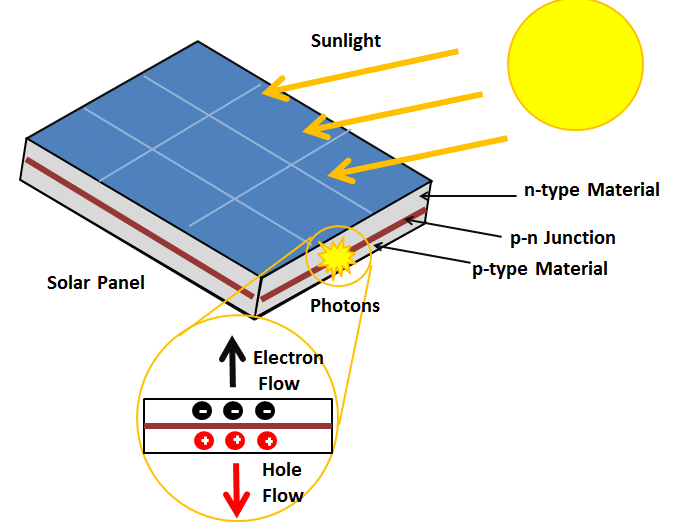
\includegraphics[width=0.4\textwidth]{figures/chap1/pv-effect.png}
    \caption{Photovoltaic Effect }
    \label{fig:pv-effect}
\end{figure}

\subsection{Components of a Photovoltaic System}
\label{sec:pv-components}

A photovoltaic system comprises several functional components designed to capture, regulate, convert, and distribute electrical energy safely \citep{franklinSolarPhotovoltaicPV}. The main components are detailed below.

\textbf{Solar Modules and Arrays:} The solar module is the foundational element that captures sunlight using multiple interconnected mono-crystalline or poly-crystalline silicon cells. To meet higher voltage and power requirements, several modules are wired together in series and parallel configurations to form a larger solar array.

\begin{figure}[H]
    \centering
    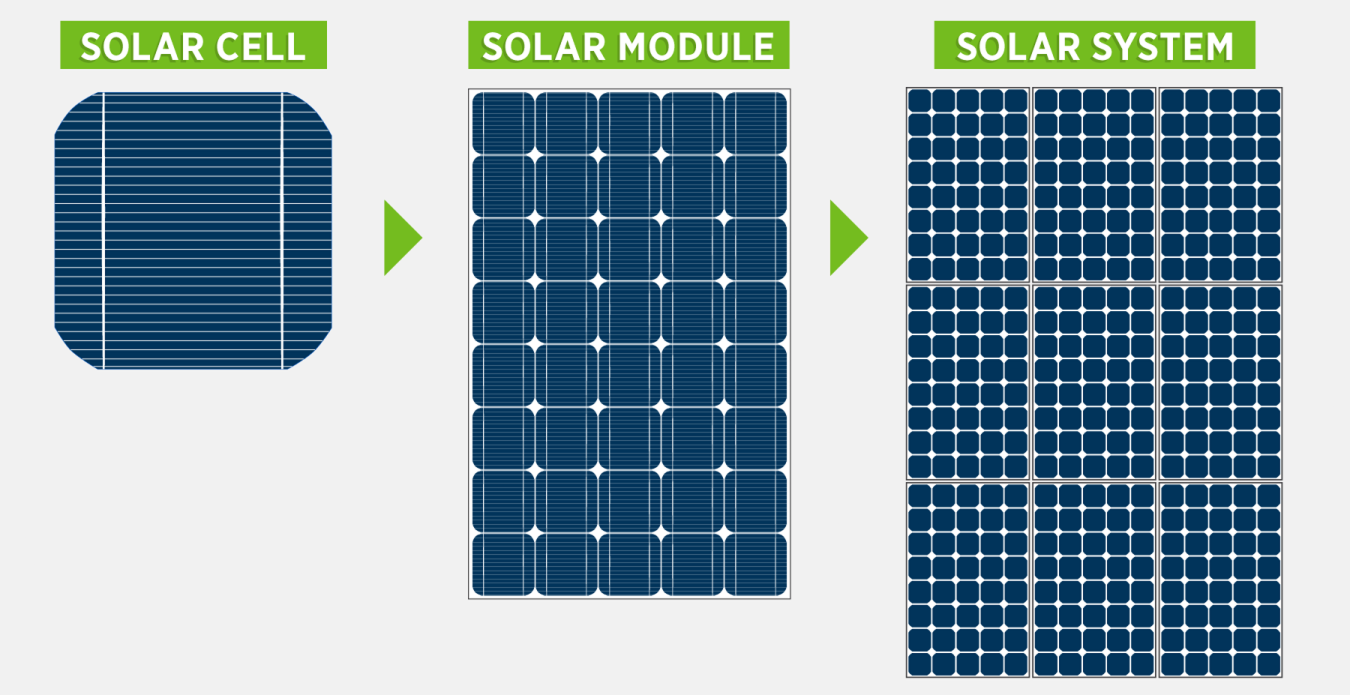
\includegraphics[width=0.4\textwidth]{figures/chap1/solar-module.png}
    \caption{The solar cell, module and array hierarchy \citep{doe2019pvcells101}}
    \label{fig:pv-components}
\end{figure}

\textbf{Combiner Box:} This electrical enclosure aggregates multiple series strings of solar modules into a single parallel output circuit. By consolidating these connections, the combiner box efficiently increases the total system current while maintaining the accumulated voltage of the strings.

\begin{figure}[H]
    \centering
    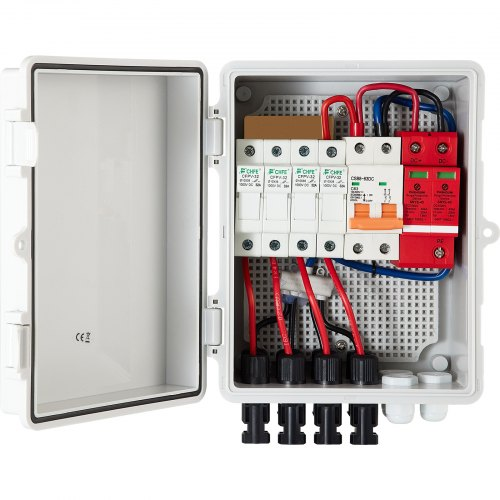
\includegraphics[width=0.3\textwidth]{figures/chap1/combiner-box.png}
    \caption{VEVOR PV Combiner Box for 4 Strings}
    \label{fig:combiner-box}
\end{figure}

\textbf{Charge Controller:} Positioned between the solar array and the battery bank, the charge controller regulates the incoming direct current. It plays a critical role in preventing battery overcharging and excessive discharging, thereby safely extending the operational lifespan of the storage system.
\begin{figure}[H]
    \centering
    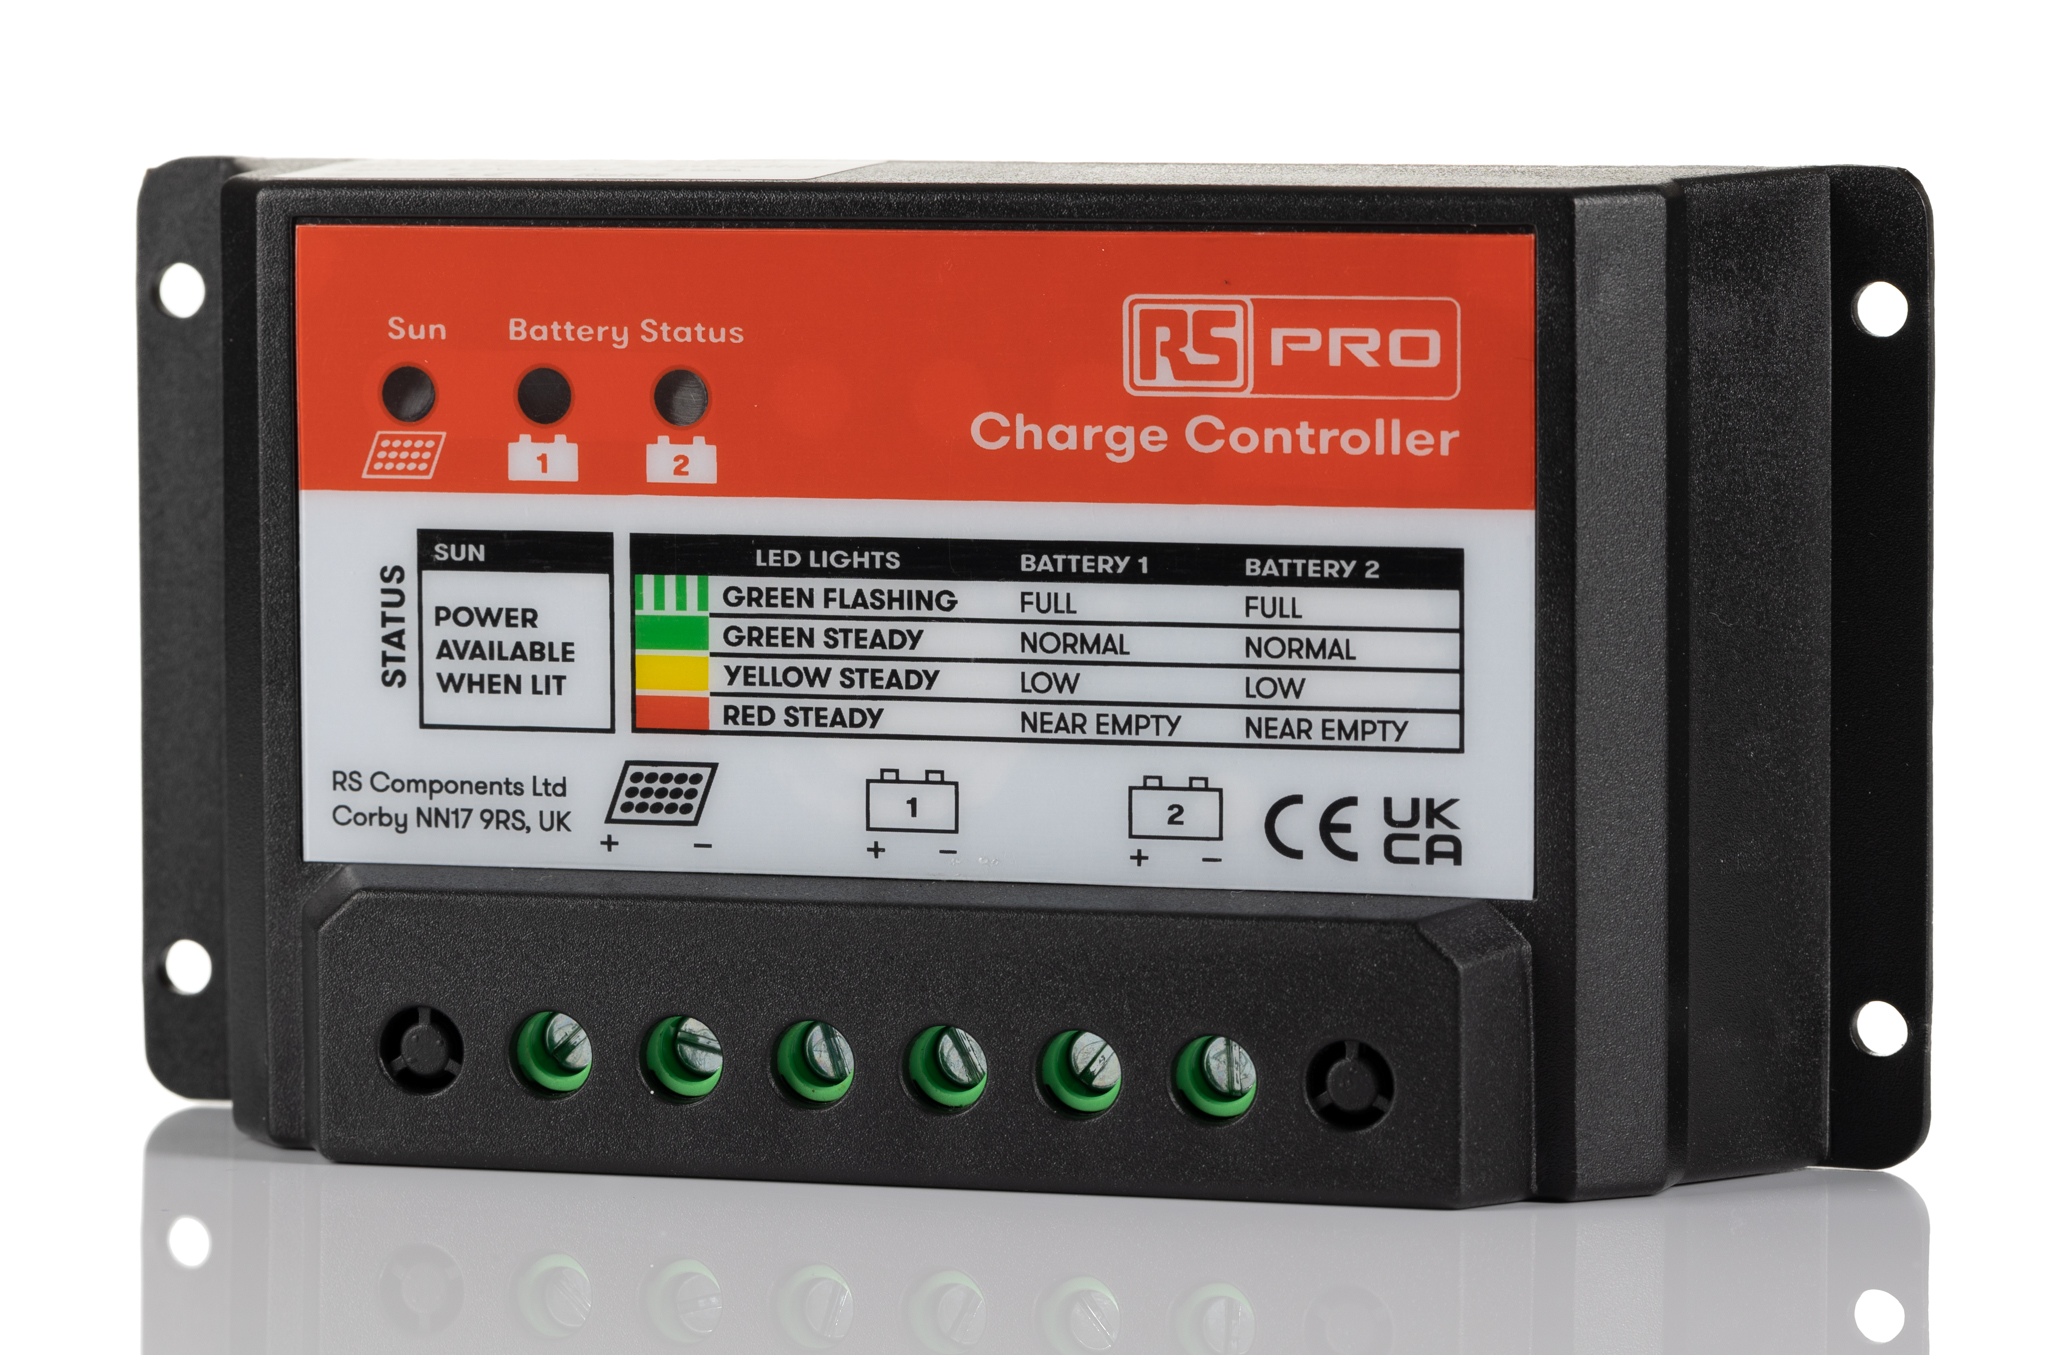
\includegraphics[width=0.3\textwidth]{figures/chap1/charge-controller.png}
    \caption{RS PRO Solar Charge Controller (24V/10A)}
    \label{fig:charge-controller}
\end{figure}
\textbf{Battery Bank:} In systems requiring energy storage, deep-cycle lead-acid batteries are utilized to store the electrical power produced during sunny periods. These batteries provide a reliable energy reserve to continuously power electrical loads during the night or periods of low solar irradiance.

\textbf{Inverter:} The inverter is a crucial power electronics device that converts the direct current generated by the array or stored in batteries into alternating current (AC). This conversion is essential because most residential and commercial electrical loads, as well as the external utility grid, operate exclusively on alternating current.
\begin{figure}[H]
    \centering
    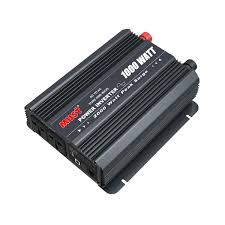
\includegraphics[width=0.3\textwidth]{figures/chap1/inverter.png}
    \caption{PI1500 Solar Power Inverter (120V 1000W)}
    \label{fig:inverter}
\end{figure}
\textbf{Disconnect Switches and Breakers:} Direct and alternating current disconnect switches are installed to safely isolate the power sources and the inverter during routine maintenance. These safety mechanisms ensure that the system can be completely de-energized, protecting the functional equipment and the maintenance personnel.

\subsection{Surveillance Systems}
\label{sec:pv-surveillance}
In the PV context, survillance systems refer to the integrated hardware and software tools used to collect and monitor system data, including electrical and meteorological parameters. These system are generally composed of sensors, plus a Supervisory Control and Data Acquisition (SCADA) system that collects, processes, and visualizes the data for performance monitoring and fault detection purposes \citep{taylorEffectivenessSCADASystem2020}.

A SCADA system typically includes Feild Devices (sensors and actuators), the main sensors in a PV system are a Pyranometer to measure solar irradiance, a Thermometer for ambient temperature and an Anemometer for wind speed measurement. Electrical parameters such as voltage, current, and power are measured directly from inverters. Remote Terminal Units are responsible for gathering data from sensors,
Master Terminal Units act as central nodes, collecting data from RTUs and providing interfaces for human operators. The collected data is also stored in a database for historical analysis \citep{yadavArchitectureSecuritySCADA2021}. An example of a SCADA system for PV monitoring can be seen in Figure~\ref{fig:scada-pv}.

\begin{figure}[H]
    \centering
    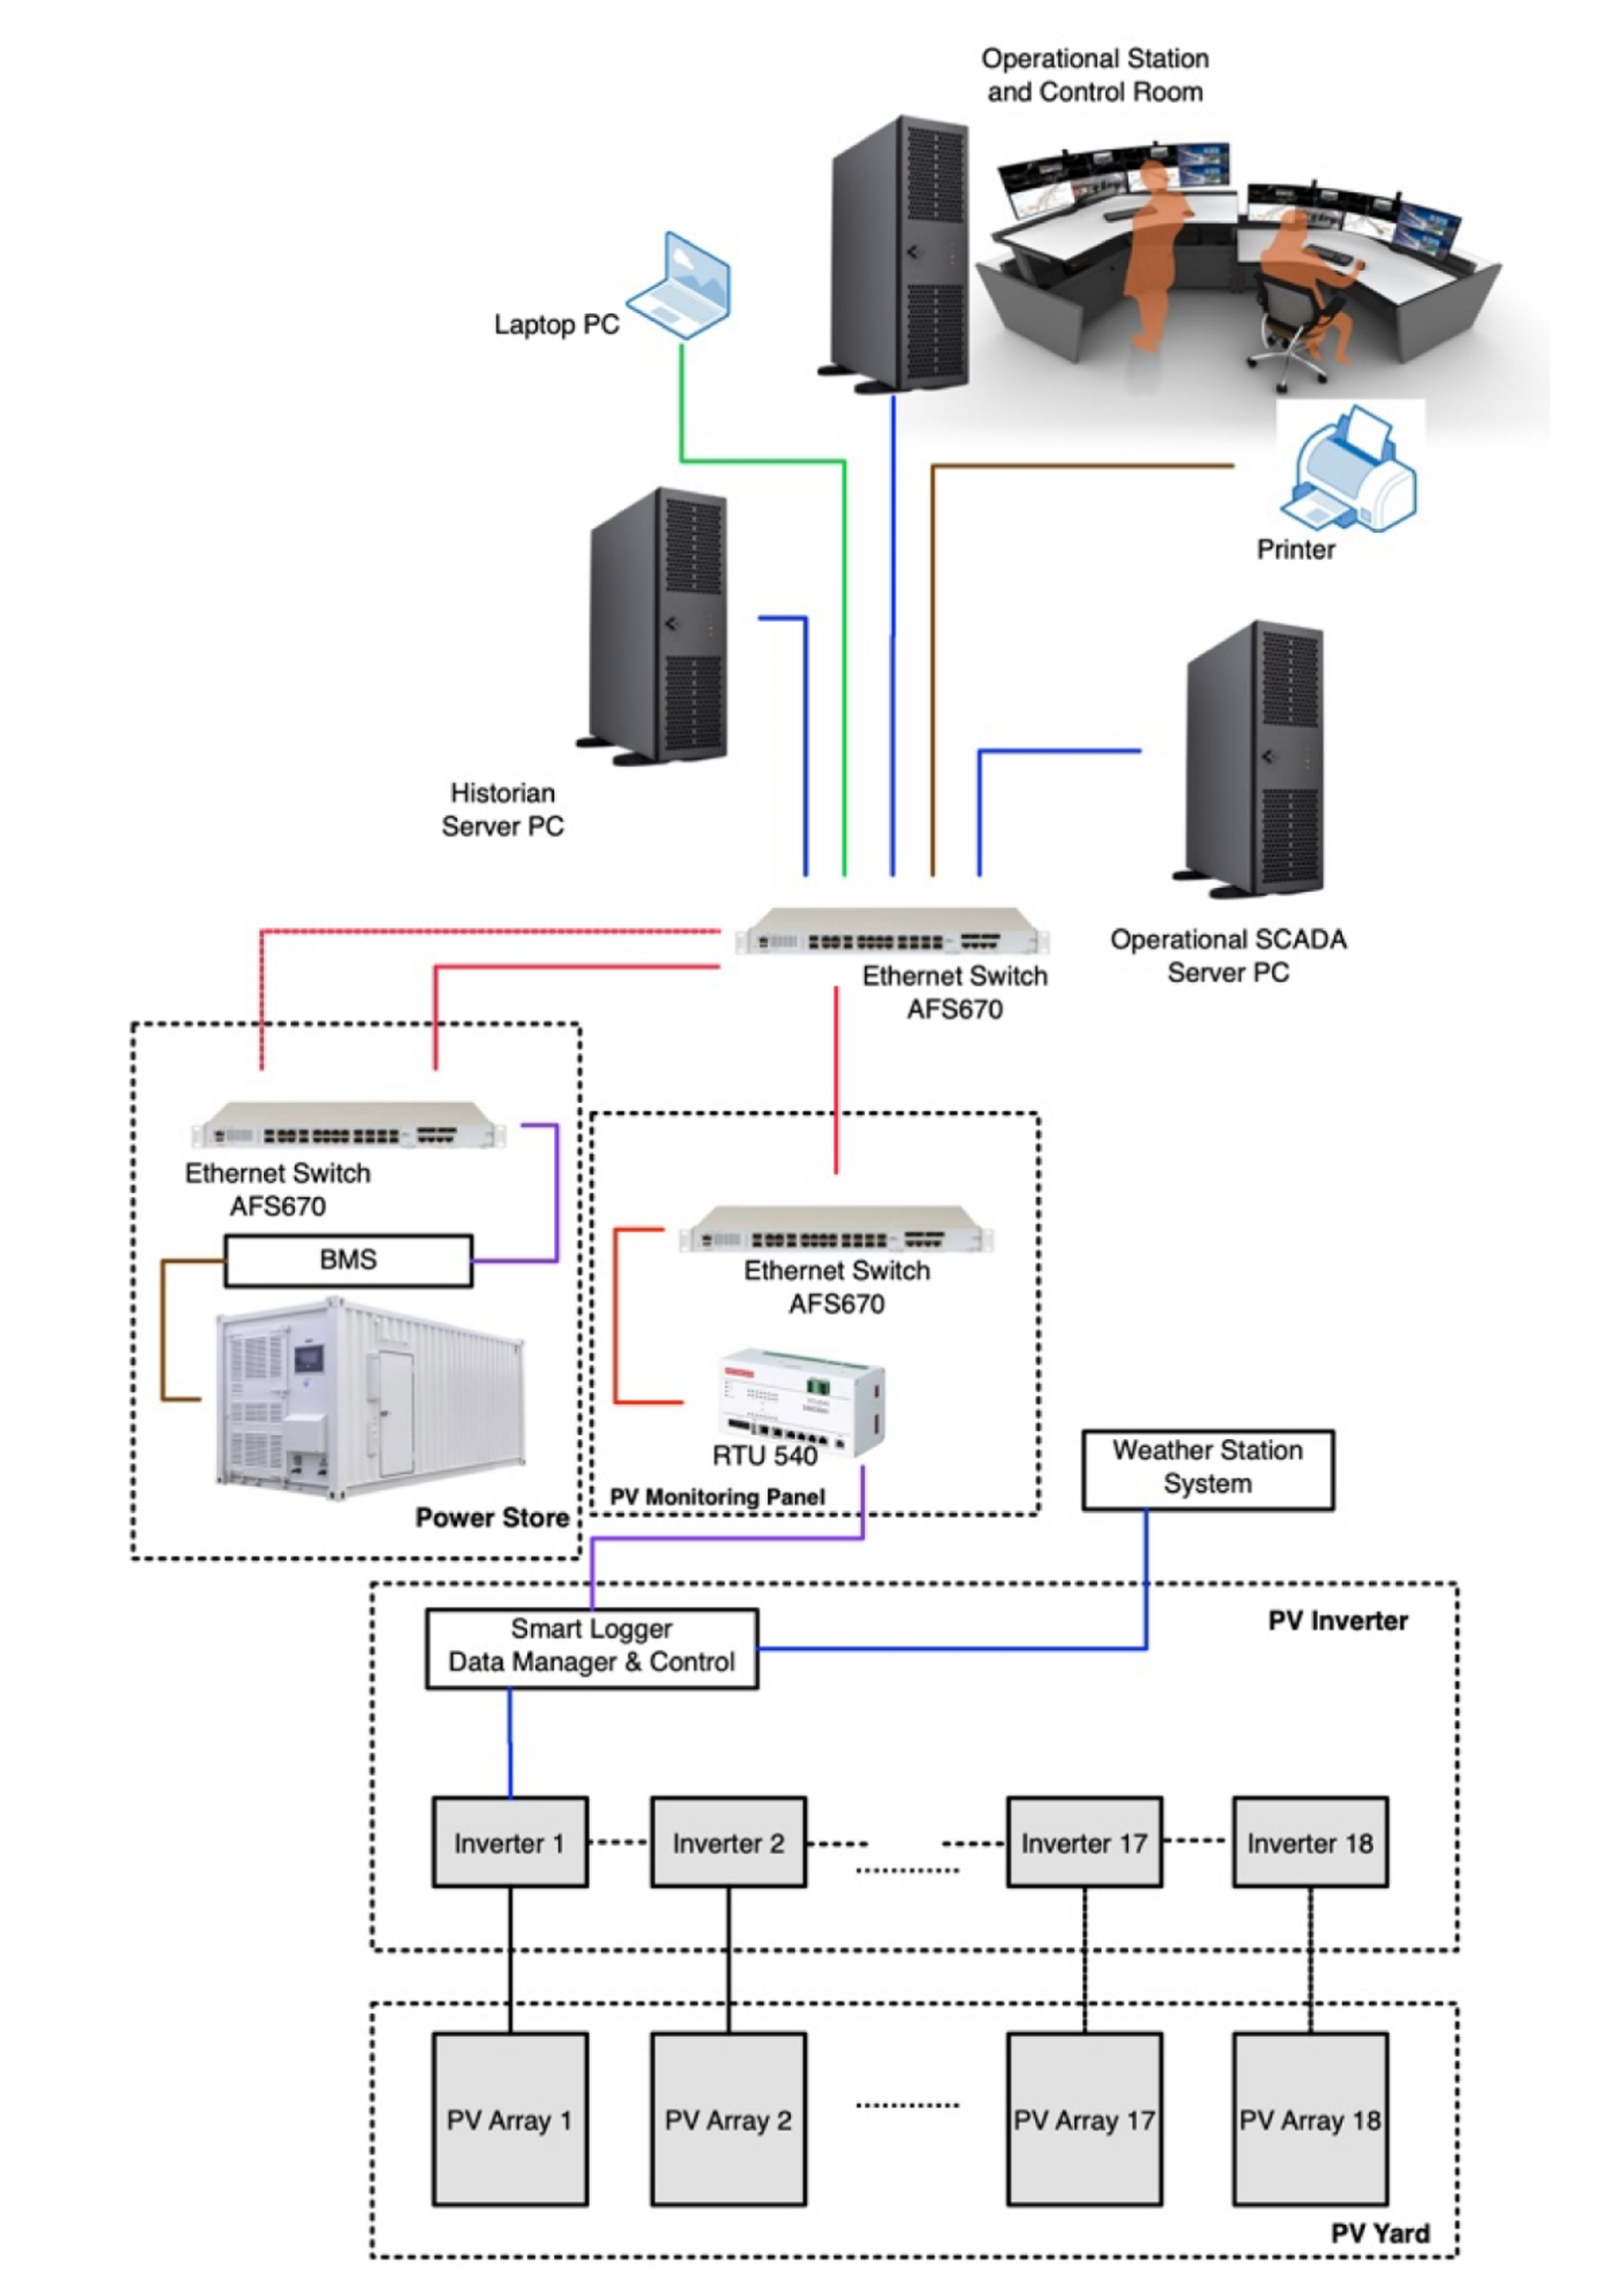
\includegraphics[width=0.7\textwidth]{figures/chap1/SCADAex.png}
    \caption{SCADA system for PV monitoring \citep{syamsuddinPredictiveMaintenanceBased2024}}
    \label{fig:scada-pv}
\end{figure}

\subsection{Global Operation of a Photovoltaic System}
\label{sec:pv-global-operation}

The operation of a photovoltaic system begins with the conversion of solar irradiance into 
direct current at the cell and module levels. Modules are interconnected into strings and 
arrays to achieve the required voltage and power levels. The generated DC power passes 
through protection and aggregation devices, and may be regulated by a charge controller 
when energy storage is used. An inverter then converts the DC power into alternating 
current for AC loads or grid injection. System operation is continuously monitored 
through sensors and SCADA platforms, which collect meteorological and electrical 
measurements for performance supervision and fault detection.


\section{Faults in PV Systems}
\label{sec:pv-faults}

Faults in a photovoltaic systems are any abnormal condition or physical damage causing operational parameters
to deviate from their normal range, leading to reduced performance, safety hazards, or system failure.
These anomalies can be grouped into different categories based on their different characteristics. \citep{elbanbyPhotovoltaicSystemFault2023} classified them into infant failures, mid-life 
failures and wear-out failures. While \citep{ArtificialIntelligenceInternet2021} categorized them into temporal and permanent faults. \citep{ComparativeAnalysisSolar2022} divided them into AC side 
faults and DC side faults. Down below are the most pertinent faults that can occur in a PV system:
\begin{itemize}
    \item \textbf{Open Circuit Fault:} Caused by a break in electrical continuity due to damaged cables, connectors, or fuses, leading to loss of power generation in the affected string.

    \item \textbf{Short Circuit Fault:} Occurs when unintended low-impedance paths form between conductors or to ground, producing abnormal current flow and safety risks.

    \item \textbf{Mismatch Fault:} Results from differences in module electrical characteristics caused by defects, degradation, or non-uniform operating conditions such as partial shading.

    \item \textbf{Hotspot Fault:} Appears when a cell operates in reverse bias and dissipates energy as heat, potentially causing permanent thermal damage.

    \item \textbf{Bypass Diode Fault:} Arises when a bypass diode fails, either reducing module output in short-circuit mode or increasing hotspot risk in open-circuit mode.

    \item \textbf{Shading Fault:} Produced by partial obstruction of sunlight, creating current imbalance between illuminated and shaded cells.

    \item \textbf{Soiling Fault:} Caused by dust or dirt accumulation on module surfaces, reducing irradiance absorption and power generation.

    \item \textbf{Thermal Stress Fault:} Results from prolonged high temperatures that accelerate aging and degradation of module materials and interconnections.

    \item \textbf{Inverter Fault:} Occurs when the power conversion stage malfunctions, affecting DC/AC conversion, cooling, or maximum power point tracking.
\end{itemize}